
%%%%%%%%%%%%%%%%%%%% file icsc2024_template.tex %%%%%%%%%%%%%%%%%%%%%
% based on icsc2017 / 2022 template updated by Alex Hofmann for icsc2024 -- Nov. 2023
%
% This is the LaTeX source for the instructions to authors using
% the LaTeX document class 'llncs.cls' for contributions to
% the Lecture Notes in Computer Sciences series.
% http://www.springer.com/lncs       Springer Heidelberg 2006/05/04
%
% It may be used as a template for your own input - copy it
% to a new file with a new name and use it as the basis
% for your article.
%
% NB: the document class 'llncs' has its own and detailed documentation, see
% ftp://ftp.springer.de/data/pubftp/pub/tex/latex/llncs/latex2e/llncsdoc.pdf
%
%%%%%%%%%%%%%%%%%%%%%%%%%%%%%%%%%%%%%%%%%%%%%%%%%%%%%%%%%%%%%%%%%%%


\documentclass[runningheads,a4paper]{llncs}

\usepackage{amssymb}
\setcounter{tocdepth}{3}
\usepackage{graphicx}
% \usepackage{url}
\usepackage{hyperref}
\usepackage[margin=1.1in]{geometry}
\hypersetup{hidelinks}
\newcommand{\keywords}[1]{\par\addvspace\baselineskip
\noindent\keywordname\enspace\ignorespaces#1}

\pagestyle{headings}

\begin{document}

\mainmatter  % start of an individual contribution

% first the title is needed
\title{cloud-5:\\A System for Composing and Publishing Cloud Music}

% a short form should be given in case it is too long for the running head
\titlerunning{Cloud Music}


% TO GARANTEE THE DOUBLE BLIND REVIEW PROCESS, PLEASE
% KEEP THESE GENERIC AUTHOR NAMES AND INSTITUTIONS

\author{AuthorA\inst{1} \thanks{I thank Dan Derks for introducing me to Tidal Cycles and Felix Roos for answering Strudel questions.}}
%
% if the names of the authors are too long for the running head, please use the format: AuthorA et al.
\authorrunning{AuthorA}

% the affiliations are given next; don't give your e-mail address
% unless you accept that it will be published
\institute{InstituteA \\ \email{your.email@yourdomain.com}}

%
% NB: a more complex sample for affiliations and the mapping to the
% corresponding authors can be found in the file "llncs.dem"
% (search for the string "\mainmatter" where a contribution starts).
% "llncs.dem" accompanies the document class "llncs.cls".
%

\maketitle
% Should be 150 to 350 words.
\begin{abstract}
    
The advent of the World Wide Web, adequate support for computer graphics and audio in HTML, and the introduction 
of WebAssembly as a low-level language and browser-hosted runtime for any number of computer language compilers, have now created an environment well suited to the \emph{online} production, publication, and presentation of music, visual music, and 
related media at a professional standard of technical quality. A piece of music on the World Wide Web no longer need be merely 
a link to a downloadable soundfile or video, or even to a stream. A piece can, indeed, be its own ``app" that is live code running at near native speed  in the listener's Web browser. I call this kind of music \emph{cloud music} because it exists only in the ``cloud,'' the omnipresent computing infrastructure of the Web. I argue that this creates an entirely new environment for music that, in the future, should be developed with its own social context and to function as an alternative means of disseminating music in addition to live performances, discs, streams, and downloads. Here, I present and demonstrate \emph{cloud-5}, a system of Web components for producing cloud music including, among other things, fixed medium music, music that plays indefinitely, visuals that generate music, music that generates visuals, interactive music, and live coding. cloud-5 includes a WebAssembly build of the sound programming language and software synthesis system Csound, a WebAssembly build of the CsoundAC library for algorithmic composition including chords, scales, and voice-leading, the live coding system Strudel, and supporting code for menus, event handlers, GLSL shaders, and more. A cloud-5 piece thus exists as an HTML page that embeds Csound code and/or score generation code and/or Strudel code and/or GLSL code, in the context of a static Web site that can be served either locally (for composing and performing) or remotely on the World Wide Web (for publication). cloud-5 differs from related online music systems  not only by incorporating Csound and CsoundAC, but even more by being designed primarily as a new medium of presentation, performance, and publication.

\keywords{html5, webassembly, csound, algorithmic composition, visual music, live coding}
\end{abstract}

\section{Introduction}

The World Wide Web was invented for instantly sharing scientific information between scientists \cite{www}. It was then co-opted by American businesses for the purpose of selling to consumers \cite{gore}. Along the way, it became a conduit for the wholesale theft of intellectual property in the form of illegal downloads of music, films, and computer games --- bad enough, but the commercial and legal reactions may well have been worse \cite{freeculture}. Then it became the platform for social media, which provide free services and entertainment to consumers in return for selling personal data to advertisers \cite{socialmedia}. Indeed, most users of the Web have increasingly been funneled through Google search and various social media platforms, which are highly proprietary, far from open, and legally and politically contested \cite{surveillance}. 

\emph{And yet}, at every step along this tortuous path, the original inventions that created the World Wide Web, including packet-switched networking (especially TCP/IP) and the Web browser itself, loosely termed ``Web standards" but in fact consisting of numerous standards from the Internet Engineering Task Force \cite{ietf}, the World Wide Web Consortium \cite{w3c}, Ecma \cite{ecma}, and other bodies, have remained non-proprietary, decentralized, backwards compatible, and more or less open. These are the many standards that are implemented by up to date Web browsers such as Firefox, Google Chrome, and so on \cite{html5test}  (fortunately, users of cloud-5 usually need consult only Csound \cite{csoundreference} \cite{csoundapireference}, CsoundAC \cite{csoundacreference}, Strudel \cite{strudel}, JavaScript \cite{javascriptreference}, and WebGL \cite{webglreference}). In fact, driven by competitive pressures to show ever more appealing ads, the power of Web browsers has increased to the point of providing the equivalent of a game engine and an operating system, running only about 1.5 to 2.5  times as slowly as native C code \cite{wasmspeed}. 

I believe that the establishment of Web standards will be seen in the future as one of the most fortunate events of our age, because they preserve essential freedoms in the face of a remarkable (and at times illegal) level of skilled greed (I remain wary, however, that private interests will end up hijacking these standards and manipulating them to be less open).

Now to music. Music now has, in spite of everything, thanks to Web standards and the growing capabilities of browsers, a new platform that provides both novel power to composers, and novel availability to audiences. This is what I call \emph{cloud music}: computer music that runs in Web browsers. Not downloads, not streams, but autonomous programs that synthesize music and visuals in real time with the option of interacting with the audience, performing endlessly, producing endless variations, and communicating across the world. Such music can be free, or secured for paid subscriptions, or supported by advertising. 

For just a few examples of cloud music, one may look to Generative.fm \cite{alexbainter}, WebSynth \cite{websynth}, Gibber \cite{gibber}, the Strudel live coding system \cite{strudel}, or my own compositions produced using the subject of this paper, cloud-5 \cite{cloud5}.

\section{Uses}

Audio resolution in cloud-5 is the same as that of WebAudio: 48,000 frames per second of float samples in 128 frame chunks \cite{webaudiostandard}. Although studio software can offer even higher resolution, WebAudio operates within the recognized range of professional audio production quality \cite{katz} \cite{bassal}.

\begin{description}
\item[Composition] The cloud-5 system contains all the astonishing capabilities already built into every standard Web browser, a complete WebAssembly build of Csound, a complete WebAssembly build of the CsoundAC algorithmic composition library, the complete Strudel live coding system which can render audio using either Csound or its own built-in sampler and synthesizer, and any other module that will run in a Web browser. All of these facilities are completely cross-platform. That makes cloud-5 far and away the easiest computer music system of comparable power to install and configure: unzip it somewhere and run a local Web server in that directory. 
\item[Fixed Pieces] These are similar to fixed medium pieces of electroacoustic music. When the user starts the piece, it plays until the score ends. 
\item[Always-On Pieces] Similar to fixed pieces; but once started, always-on pieces play indefinitely. Using randomization or chaos, always-on pieces can play indefinitely without any repetition.
\item[Interactive Pieces] Similar to fixed pieces or always-on pieces; but once the piece is started, the user interface provides controls with which the user may steer some aspects of the composition or rendering.
\item[Live Coding] Similar to interactive pieces; but the user has \emph{complete} control over the composition in the Strudel REPL, and can create entirely new compositions or engage in lengthy improvisations.

\item[Music Visualization] Similar to the other pieces above, but a GLSL shader displays a visualization controlled by the audio on the background of the piece; this visualization can be made full screen.
\item[Visual Music] Similar to music visualization, but the video buffer is periodically downsampled or otherwise processed to produce fragments of Csound score, which are rendered by Csound in real time.
\item[Network Pieces] Any of these types of pieces can request additional resources from the Internet, or be controlled remotely.
\end{description}

\section{Design}

The cloud-5 user interface consists of a main menu running across the top of the page. Clicking on a button can start or stop performance, or show/hide various overlays that fill the rest of the page. 

\begin{figure}
\centering
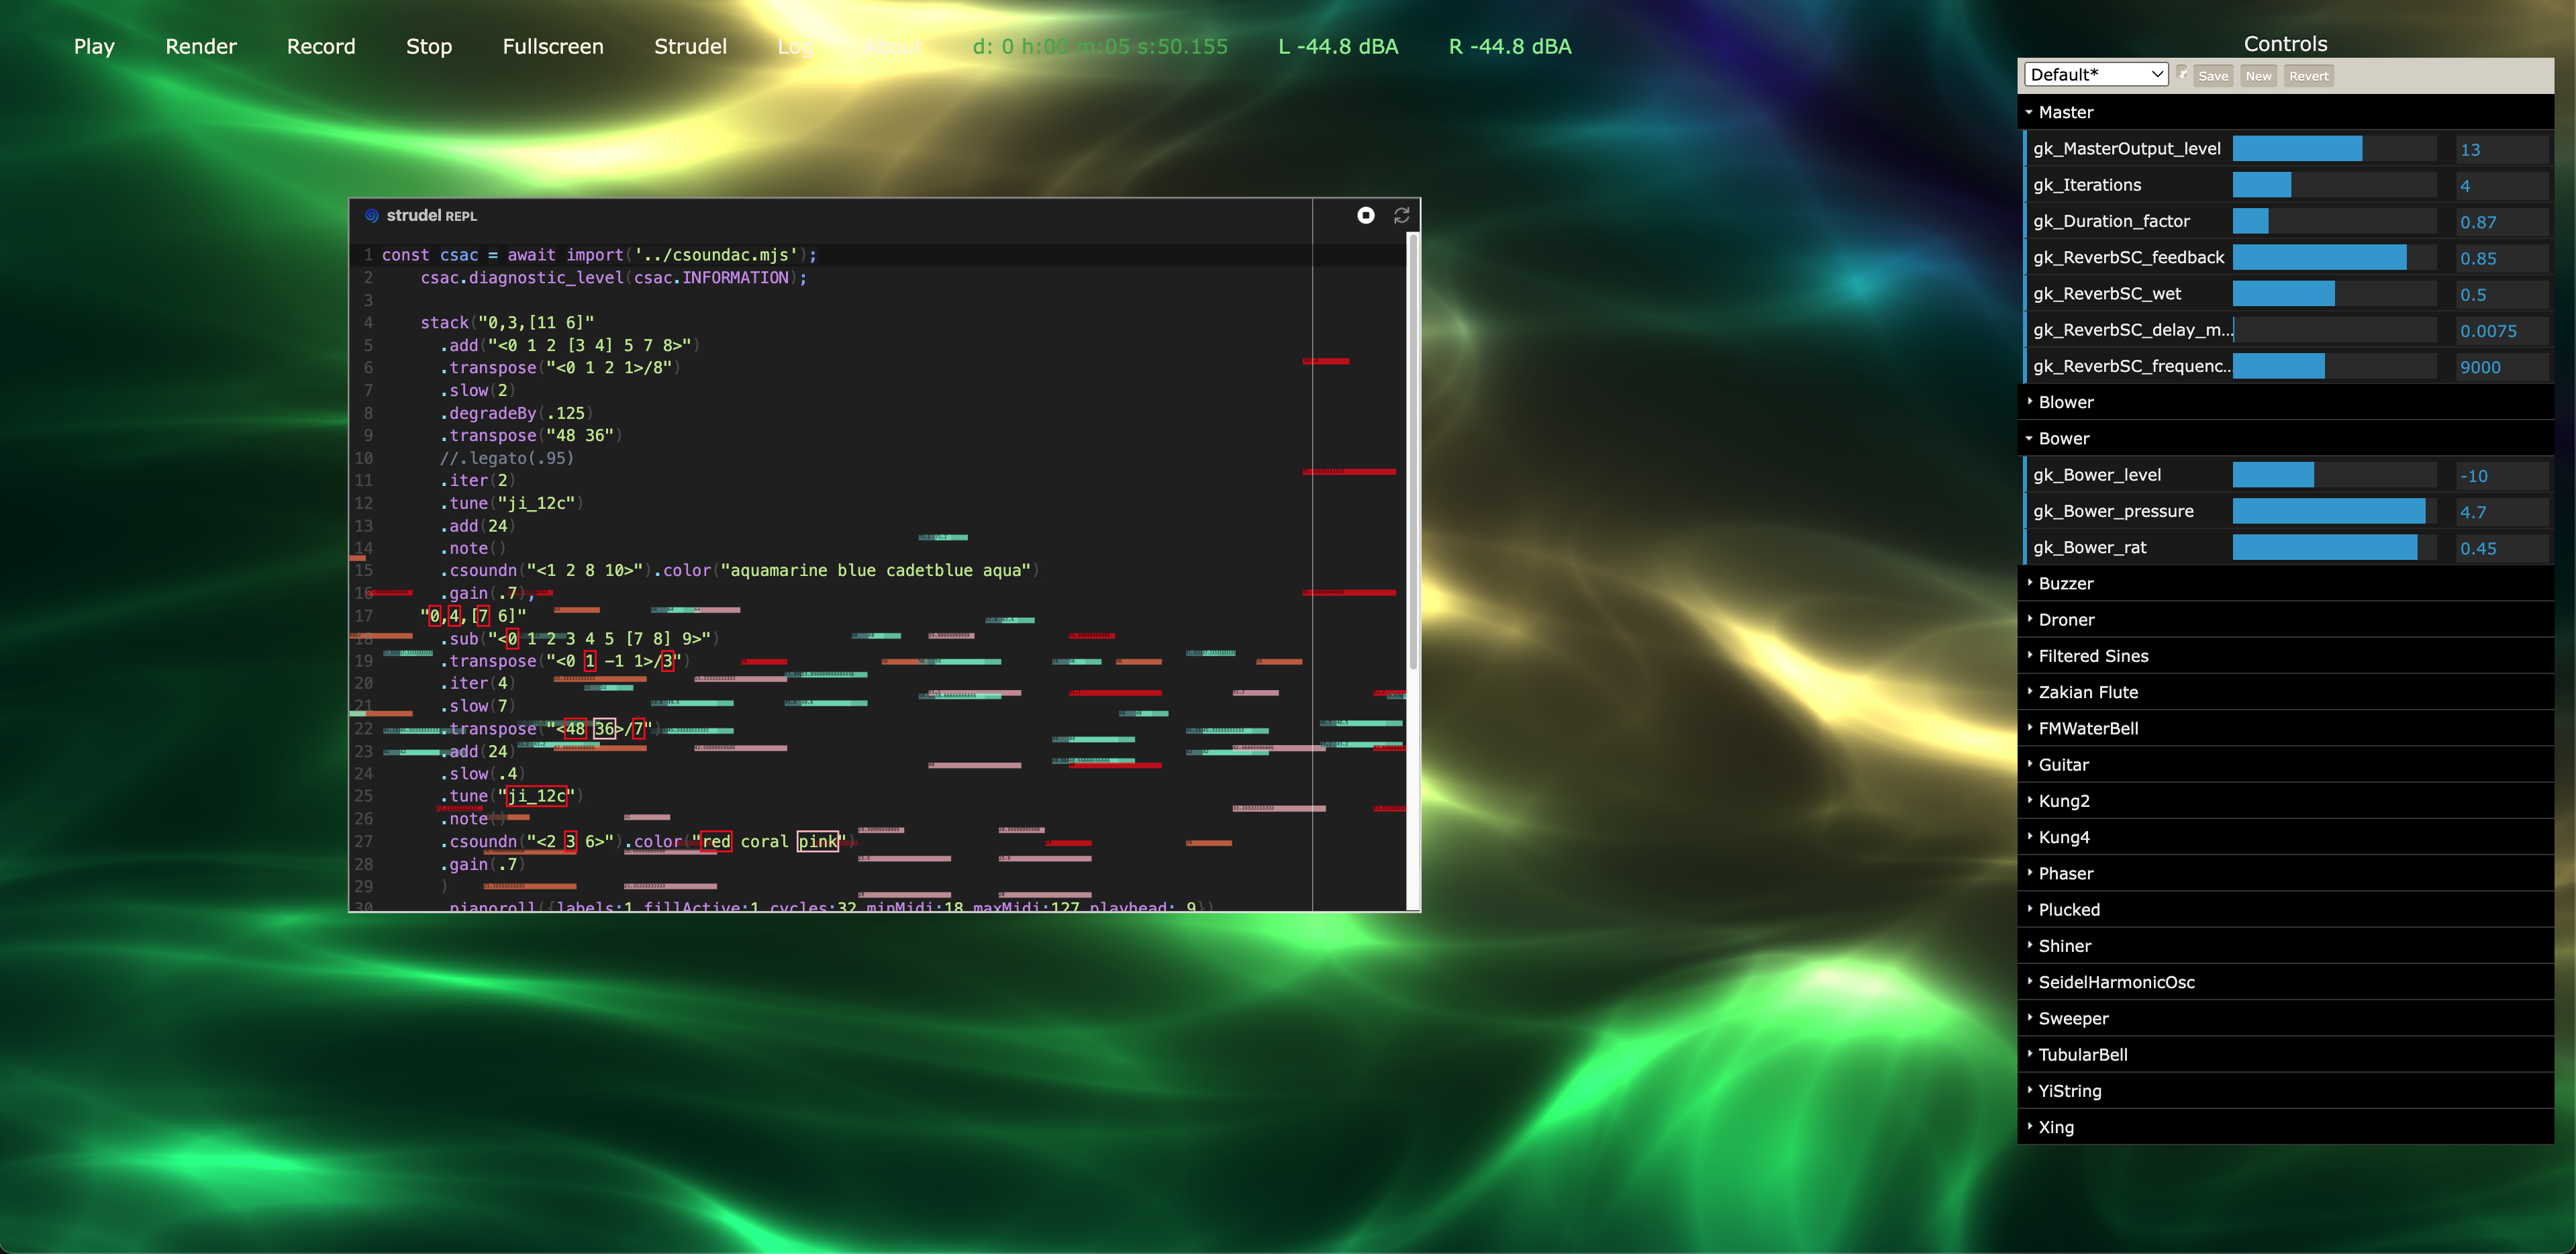
\includegraphics[width=0.90\linewidth]{cloud5}
\caption{cloud-5 Piece with Strudel and Audio Visualization}
\label{fig:cloud5}
\end{figure}

The system is constructed as a library of HTML custom elements, which encapsulate code and even some styling within each custom element. That makes it much easier for users not familiar with the details of HTML or JavaScript to compose cloud-5 pieces. The user includes these custom elements in their HTML code like any other elements, adds user-defined code such as a Csound orchestra or Strudel patch, and hooks the parts up together using a little JavaScript. Code folding regions make it easier to organize the code and to see only the part that is being edited. 

Currently, cloud-5 consists of a number of custom elements and user addons. To make it easier for users to construct pieces, names ending in \texttt{\_overlay} denote Web components, and names ending in \texttt{\_addon} denote things that the user must or may provide, including code (JavaScript, Csound, Strudel, GLSL), parameters, and others.

\begin{description}
\item[\texttt{<cloud5-piece>}] Defines the main menu of the piece, instantiates Csound and/or Strudel as required, starts and stops performances, hosts a controls menu, and defines some helper JavaScript code.
\item[\texttt{<cloud5-piece>.csound\_code\_addon}]  A JavaScript string literal containing user-defined source code for a Csound .csd file (which can be quite large).
\item[\texttt{<cloud5-piece>.control\_parameters\_addon}]  A user-defined JavaScript object whose fields have the names and initial values of Csound control channels.
\item[\texttt{<cloud5-piece>.menu\_folder\_addon}]  The user calls this with the name of a new folder to be added to the controls menu of the piece.
\item[\texttt{<cloud5-piece>.menu\_slider\_addon}]  The user calls this to create a new new slider control in a folder, specifying its Csound channel name, lowest value, and highest value.
\item[\texttt{<cloud5-piece>.score\_generator\_function\_addon}]  A user-defined JavaScript function that will be called at the start of performance to generate a CsoundAC score for performance by Csound. 
\item[\texttt{<cloud5-piano-roll>}] An overlay that draws a three-dimensional piano roll display of a generated score. During performance, the piano roll shows the current position in the score with a moving ball. It is possible to zoom in and out of the piano roll, drag it around, rotate it, and so on.
\item[\texttt{<cloud5-strudel>}] A popup IFrame that shows the Strudel REPL, in which the user can do live coding of the Strudel patch during performance. The Strudel REPL has its own real-time piano roll display, and highlights the currently active functions in the Strudel code.
\item[\texttt{<cloud5-strudel>.strudel\_code\_addon}] A JavaScript string literal containing a user-defined  Strudel patch to perform the piece.
\item[\texttt{<cloud5-shadertoy>}] An overlay that shows a canvas displaying a GLSL shader. This shader can be used to visualize audio, to produce notes for Csound to perform, and so on. The element is designed to support the easy adaptation of shaders developed in the ShaderToy Web site \cite{shadertoy}.
\item[\texttt{<cloud5-shadertoy>.shader\_parameters\_addon}] A user-defined Javascript object with the following fields:
\begin{description}
\item[\texttt{fragment\_shader\_code\_addon}] A JavaScript string literal containing user-defined GLSL code to be compiled for display on the canvas of the shader overlay.
\item[\texttt{vertex\_shader\_code\_addon}] May contain user-defined GLSL code to be compiled for display on the canvas of the shader overlay; there is a default value that includes the entire canvas.
\item[\texttt{pre\_draw\_frame\_function\_addon}] May be set to user-defined code in the form of a JavaScript function that will be called just before drawing each shader animation frame, e.g. to set uniforms that control the shader; commonly used to implement an audio visualizer.
\item[\texttt{post\_draw\_frame\_function\_addon}] This may be set to user-defined code in the form of a JavaScript function that will be called just after drawing each shader animation frame, e.g. to sample the visuals and translate them to Csound notes to be played.
\end{description}
\item[\texttt{<cloud5-log>}] An overlay that presents a scrolling list of runtime messages from Csound and/or other sources.
\item[\texttt{<cloud5-about>}] An overlay that presents license information, authorship, credits, program notes, and so on.
\end{description}

\section{Assembling a Piece}

The following code outline shows how the components of a cloud-5 piece may be assembled, as implemented in a \verb|<script>| element of a piece:

\begin{verbatim}
<script>
    let cloud5_piece = document.querySelector("cloud5-piece");
    cloud5_piece.csound_code_addon = document.querySelector("#csd").textContent;
    cloud5_piece.score_generator_function_addon = async function () {
      // User-defined source code here.
    };
    cloud5_piece.strudel_overlay = document.querySelector("cloud5-strudel");
    cloud5_piece.strudel_overlay.strudel_code_addon = 
        document.querySelector("#strudel-code").textContent;
    cloud5_piece.control_parameters_addon = {
        "gk_MasterOutput_level": -7,
    };
    let Master = cloud5_piece.menu_folder_addon("Master");
    cloud5_piece.menu_slider_addon(Master, "gk_MasterOutput_level", -50, 50);
    let cloud5_piano_roll = document.querySelector("cloud5-piano-roll");
    cloud5_piece.piano_roll_overlay = cloud5_piano_roll;
    let fragment_shader = document.getElementById("draw-shader-fs").textContent;
    cloud5_shader.shader_parameters_addon = {
        fragment_shader_code_addon: fragment_shader,
    };
    cloud5_piece.shader_overlay = cloud5_shader;
    let cloud5_log = document.querySelector("cloud5-log");
    cloud5_piece.log_overlay = cloud5_log;
    let cloud5_about = document.querySelector("cloud5-about");
    cloud5_piece.about_overlay = cloud5_about;
</script>
\end{verbatim}

\section{Best Practices}

The cloud-5 system is designed for creating permanent works of music -- pieces that will always play, even in the far future (assuming that Web standards continue to be versionless and backwards-compatible, as they have been for 35 years). In other words, cloud-5 is not at all a general purpose Web development system, and therefore pieces should not be developed in the standard way.

\begin{itemize}
\item Use only local, static resources (e.g., do not use content distribution networks, but rather download all required scripts, etc., to the Web directory). This ensures pieces will continue to function indefinitely, and will not break due to library API changes or missing links.
\item Use no tooling (e.g. no rollups); edit pieces directly in the Web directory. This ensures that pieces will not break due to tooling changes, and will be easy to debug.
\item As far as possible, keep all components and resources of a piece in one HTML file, e.g. embed Csound orchestras and Strudel patches in the HTML code.
\end{itemize}

\noindent Live examples of cloud-5 pieces may be found at \url{https://AuthorA.github.io/}, source code and binary releases may be found at \url{https://github.com/AuthorA/cloud-5}.

\begin{thebibliography}{4}

\bibitem{socialmedia} Mandiber, Michael: The Social Media Reader. New York: NYU Press (2012).

\bibitem{wasmspeed} Jangda, Abhinav, Bobby Powers, Emery D. Berger, and Arjun Guha. Not So Fast: Analyzing the Performance of WebAssembly vs. Native Code. \url{https://arxiv.org/abs/1901.09056} (2019).

\bibitem{www} Isacson, Walter: The Innovators: How a Group of Hackers, Geniuses, and Geeks Created the Digital Revolution. New York: Simon and Schuster (2015).

\bibitem{gore} Hafner, Katie and Matthew Lyon: Where Wizards Stay Up Late: The Origins of the Internet. New York: Simon and Schuster (1998).

\bibitem{surveillance} Zuboff, Shoshona: The Age of Surveillance Capitalism. New York: Public Affairs (2019).

\bibitem{freeculture} Lessig, Lawrence: Free Culture: How Big Media Uses Technology and the Law to Lock Down Culture and Control. City of Westminser: Penguin Books (2004).

\bibitem{webglreference} Mozillla Developer Network: WebGL Reference. \url{https://developer.mozilla.org/en-US/docs/Web/API/WebGL_API} Accessed 24 March 2024).

\bibitem{playcanvas} \url{https://playcanvas.com/} (Accessed 23 March 2024).

\bibitem{ecma} Ecma: Emca International. \url{https://ecma-international.org} (Accessed 23 March 2024).

\bibitem{w3c} W3C: Making the Web work. \url{https://www.w3.org} (Accessed 23 March 2024).

\bibitem{ietf} Internet Engineering Task Force: I E T F \url{https://www.ietf.org} Accessed 23 March 2024).

\bibitem{html5test} HTML 5 Test: \url{https://html5test.co} (Accessed 23 March 2024).

\bibitem{httpstandard} IETF: HTTP Semantics \url{https://www.rfc-editor.org/info/rfc9110} (June 2022).

\bibitem{w3cstandards} W3C: Web Standards. \url{https://www.w3.org/standards} (Accessed 23 March 2024).

\bibitem{webaudiostandard} W3C: Web Audio API. \url{https://webaudio.github.io/web-audio-api} (11 March 2024).

\bibitem{csoundapireference} Csound Developers: Csound API 6.18. \url{https://csound.com/docs/api/index.html} (Accessed 23 March 2024).

\bibitem{csoundacreference} Gogins, Michael: Csound AC 1.0.0 \url{https://github.com/gogins/csound-ac/blob/master/csound-ac.pdf} (Accessed 23 March 2024).

\bibitem{csoundreference} Csound Community: The Canonical Csound Reference Manual, Version 6.18.0 \url{https://csound.com/docs/manual/index.html} (Accessed 23 March 2024).

\bibitem{javascriptreference} Mozilla Developer Network: JavaScript Reference. \url{https://developer.mozilla.org/en-US/docs/Web/JavaScript/Reference} (Accessed 24 March 2024).

\bibitem{katz} Katz, Robert A.. Mastering Audio: The Art and the Science, Third Edition. Netherlands: Focal Press (2015).

\bibitem{bassal} Bassal, Dominique: The Practice of Mastering in Electroacoustics. \url{https://cec.sonus.ca/pdf/The\_Practice\_of\_Mastering.pdf} (December 2002).

\bibitem{book2} lazzarini, V. et al.: Csound: A Sound and Music Computing System.
Springer (2016)

\bibitem{url} Csound Github site, \url{http://csound.github.io}.

\bibitem{alexbainter} Bainter, Alex: web. music.
generative art. \url{https://alexbainter.com} (Accessed 23 March 2024).

\bibitem{strudel} Roos, Felix, Alex McLean, et al.: Strudel REPL. \url{https://strudel.cc/} (Accessed 23 March 2024).

\bibitem{cloud5} cloud-music: Computer Music on the Web \url{https://AuthorA.github.io} (Accessed 23 March 2024).

\bibitem{websynth} Primozic, Casey: Web Synth. \url{https://synth.ameo.dev} (Accessed 24 March 2024).
 
\bibitem{gibber} Roberts, Charlie: Gibber \url{https://gibber.cc} Accessed 24 March 2024).

\bibitem{shadertoy} Quilez, Inigo, Pol Jeremias, et al.: ShaderToy BETA \url{https://www.shadertoy.com} (Accessed 24 March 2024).

\end{thebibliography}

\end{document}
